% \documentclass[11pt,twoside]{book} %纸质版用twoside
\documentclass[12pt,oneside]{book} %电子版用oneside
\usepackage{setspace}

% \documentclass{article}

%%%%%%%%%%%%%%%%%%%%%%%%%%%%%%%%%%%%%%%%%%%%%%%%%%
%%%%%%%%%%%%%%%%%%%%% preamble %%%%%%%%%%%%%%%%%%%
%%%%%%%%%%%%%%%%%%%%%%%%%%%%%%%%%%%%%%%%%%%%%%%%%%

\usepackage[mono=false]{libertine} % new linux font, ignore mono

\usepackage{luatex85}

%\renewcommand{\baselinestretch}{1.05}
\usepackage{amsmath,amsthm,amssymb,mathrsfs,amsfonts,dsfont}
\usepackage{epsfig,graphicx}
\usepackage{tabularx}
\usepackage{blkarray}
\usepackage{slashed}
\usepackage{color}
\usepackage{listings}
\usepackage{caption}
% \usepackage{fullpage}
\usepackage{lipsum} % provides dummy text for testing
\usepackage[toc,title,titletoc,header]{appendix}
\usepackage{minitoc}
\usepackage{color}
\usepackage{multicol} % two-col ToC
\usepackage{bm}
\usepackage{imakeidx} % before hyperref
\usepackage{hyperref}
\usepackage{indentfirst}
\setlength{\parindent}{2em}


% link colors settings
\hypersetup{
    colorlinks=true,
    citecolor=magenta,
    linkcolor=blue,
    filecolor=green,      
    urlcolor=cyan,
    % hypertexnames=false,
}
\usepackage[capitalise]{cleveref}
\usepackage{subcaption}
\usepackage{enumitem}
\usepackage{mathtools}
\usepackage{physics}
\usepackage[linesnumbered,ruled,vlined,algosection]{algorithm2e}
\SetCommentSty{textsf}
\usepackage{epigraph}
\epigraphwidth=1.0\linewidth
\epigraphrule=0pt

% adjust margin
\usepackage[margin=2.3cm]{geometry}
\headheight13.6pt


\usepackage{graphicx}
\usepackage[justification=centering]{caption} % 图注居中
\usepackage{setspace}
\usepackage{geometry}
\usepackage{float}
\usepackage{hyperref}
\usepackage[utf8]{inputenc}
\usepackage[english]{babel}
\usepackage{framed}


\newcommand{\HRule}[1]{\rule{\linewidth}{#1}}





\setstretch{1.2}
% \geometry{
%     textheight=9in,
%     textwidth=5.5in,
%     top=1in,
%     headheight=12pt,
%     headsep=25pt,
%     footskip=30pt
% }





%%%%%%%%%%%%%%%% thmtools %%%%%%%%%%%%%%%%%%%%%

\usepackage{thmtools}
\usepackage[dvipsnames]{xcolor}
\usepackage[most]{tcolorbox}
\usepackage{enumerate}

\colorlet{LightGreen}{Green!15} %def
\colorlet{LightBlue}{Blue!15} %thm
\colorlet{LightOrange}{Orange!15} %lem
\colorlet{LightGray}{Gray!15}  %prop
\colorlet{LightRed}{Red!40} %cor
\colorlet{LightYellow}{Yellow!15} %exa


% \newtcbtheorem[
%   number within = chapter % 按每个 chapter 分别编号
% ]{definition% 环境名
% }{Definition% 这个参数可以设成“定理”“引理”“推论”等,编号就会变成“定理 1.1”“引理 1.1”“推论 1.1”等
% }{
%   attach title to upper = \par\vspace{1ex}, % 不要单独的标题栏,定理名完了之后分段,加上适量空白
%   separator sign = \quad, % 定理编号和定理名字之间用什么分隔;默认是冒号
%   sharp corners, % 直角;默认是圆角
%   enhanced jigsaw, frame hidden, % 隐藏 tcb 边框
%   colback = LightGreen, % 背景色
%   coltitle = blue!20!cyan!80!black, % 标题(定理编号和名字)的颜色
%   fonttitle = \sffamily\small, % 标题(定理编号和名字)的字体
%   description font = \normalsize, % 定理名字的字体
%   fontupper = \normalfont, % box 内的字体
% }{def% label 前缀
% }

\newtcbtheorem[
  auto counter,number within = chapter % 按每个 chapter 分别编号
]{definition% 环境名
}{Definition% 这个参数可以设成“定理”“引理”“推论”等,编号就会变成“定理 1.1”“引理 1.1”“推论 1.1”等
}{
  sharp corners, % 直角;默认是圆角
  colback=Green!5,
  colframe=Green!50!black,
  fonttitle=\sffamily\small
}{def% label 前缀
}


% 计数器设置
\makeatletter
\renewcommand\theHtcb@cnt@definition{\thechapter.\arabic{tcb@cnt@definition}}
\makeatother

\newtcbtheorem[
  auto counter,number within = chapter % 按每个 chapter 分别编号
]{theorem% 环境名
}{Theorem% 这个参数可以设成“定理”“引理”“推论”等,编号就会变成“定理 1.1”“引理 1.1”“推论 1.1”等
}{
  sharp corners, % 直角;默认是圆角
  colback=yellow!10,
  colframe=yellow!50!black,
  fonttitle=\sffamily\small
}{thm% label 前缀
}
% 计数器设置
\makeatletter
\renewcommand\theHtcb@cnt@theorem{\thechapter.\arabic{tcb@cnt@theorem}}
\makeatother

\newtcbtheorem[
  auto counter,number within = chapter % 按每个 chapter 分别编号
]{proposition% 环境名
}{Proposition% 这个参数可以设成“定理”“引理”“推论”等,编号就会变成“定理 1.1”“引理 1.1”“推论 1.1”等
}{
  sharp corners, % 直角;默认是圆角
  colback=Red!5,
  colframe=Red!50!black,
  fonttitle=\sffamily\small
}{prop% label 前缀
}
% 计数器设置
\makeatletter
\renewcommand\theHtcb@cnt@proposition{\thechapter.\arabic{tcb@cnt@proposition}}
\makeatother

\newtcbtheorem[
  auto counter,number within = chapter % 按每个 chapter 分别编号
]{corollary% 环境名
}{Corollary% 这个参数可以设成“定理”“引理”“推论”等,编号就会变成“定理 1.1”“引理 1.1”“推论 1.1”等
}{
  sharp corners, % 直角;默认是圆角
  colback=Blue!5,
  colframe=Blue!50!black,
  fonttitle=\sffamily\small
}{cor% label 前缀
}

% 计数器设置
\makeatletter
\renewcommand\theHtcb@cnt@corollary{\thechapter.\arabic{tcb@cnt@corollary}}
\makeatother

\newtcbtheorem[
  auto counter,number within = chapter % 按每个 chapter 分别编号
]{lemma% 环境名
}{Lemma% 这个参数可以设成“定理”“引理”“推论”等,编号就会变成“定理 1.1”“引理 1.1”“推论 1.1”等
}{
  sharp corners, % 直角;默认是圆角
  colback=Gray!10,
  colframe=Gray!50!black,
  fonttitle=\sffamily\small
}{lem% label 前缀
}

% 计数器设置
\makeatletter
\renewcommand\theHtcb@cnt@lemma{\thechapter.\arabic{tcb@cnt@lemma}}
\makeatother


\newtcbtheorem[
  auto counter,number within = chapter % 按每个 chapter 分别编号
]{example}
{Example}%
  {
    enhanced, breakable,
    colback = white, colframe = purple, colbacktitle = purple,
    attach boxed title to top left = {yshift = -2mm, xshift = 5mm},
    boxed title style = {sharp corners},
    fonttitle=\sffamily\small
  }
{exa}

% 计数器设置
\makeatletter
\renewcommand\theHtcb@cnt@example{\thechapter.\arabic{tcb@cnt@example}}
\makeatother


\newtcbtheorem[
  auto counter,number within = chapter % 按每个 chapter 分别编号
]{exercise}
{Exercise}%
  {
    enhanced, breakable,
    colback = white, colframe = cyan, colbacktitle = cyan,
    attach boxed title to top left = {yshift = -2mm, xshift = 5mm},
    boxed title style = {sharp corners},
    fonttitle=\sffamily\small
  }
{exer}

% 计数器设置
\makeatletter
\renewcommand\theHtcb@cnt@exercise{\thechapter.\arabic{tcb@cnt@exercise}}
\makeatother


% \declaretheorem[numberwithin=chapter,shaded={rulecolor=LightGreen,
% rulewidth=2pt,bgcolor=LightGreen,
% textwidth=12em}]{definition}

\usepackage{changepage}
\newenvironment{remark}{\underline{\textbf{Remark.}}}{\par}

\newenvironment{proofsolution}
    {\renewcommand\qedsymbol{$\square$}\color{blue}\begin{adjustwidth}{0em}{2em}\begin{proof}[\textit Proof.~]}
    {\end{proof}\end{adjustwidth}}


%%%%%%%%%%%%%%%% index %%%%%%%%%%%%%%%%%%%%%
\begin{filecontents}{index.ist}
% https://tex.stackexchange.com/questions/65247/index-with-an-initial-letter-of-the-group
headings_flag 1
heading_prefix "{\\centering\\large \\textbf{"
heading_suffix "}}\\nopagebreak\n"
delim_0 "\\nobreak\\dotfill"
\end{filecontents}
\newcommand{\myindex}[1]{\index{#1} \emph{#1}}
\makeindex[columns=3, intoc, title=Alphabetical Index, options= -s index.ist]
%%%%%%%%%%%%%%%% index %%%%%%%%%%%%%%%%%%%%%

%%%%%%%%%%%%%%%% ToC %%%%%%%%%%%%%%%%%%%%%
% Link Chapter title to ToC: https://tex.stackexchange.com/questions/32495/linking-the-section-text-to-the-toc
\usepackage[explicit]{titlesec}
\titleformat{\chapter}[display]
  {\normalfont\huge\bfseries}{\chaptertitlename\ {\thechapter}}{20pt}{\hyperlink{chap-\thechapter}{\Huge#1}
\addtocontents{toc}{\protect\hypertarget{chap-\thechapter}{}}}
\titleformat{name=\chapter,numberless}
  {\normalfont\huge\bfseries}{}{-20pt}{\Huge#1}

%%%%%%%%%%%%%%%%%%% fancyhdr %%%%%%%%%%%%%%%%%
\usepackage{fancyhdr}
\pagestyle{fancy} % enable fancy page style
\renewcommand{\headrulewidth}{0.0pt} % comment if you want the rule
\fancyhf{} % clear header and footer
\fancyhead[lo,le]{\leftmark}
\fancyhead[re,ro]{\rightmark}
\fancyfoot[CE,CO]{\hyperref[toc-contents]{\thepage}}

% https://tex.stackexchange.com/questions/550520/making-each-page-number-link-back-to-beginning-of-chapter-or-section
\makeatletter
\def\chaptermark#1{\markboth{\protect\hyper@linkstart{link}{\@currentHref}{Chapter \thechapter ~ #1}\protect\hyper@linkend}{}}
\def\sectionmark#1{\markright{\protect\hyper@linkstart{link}{\@currentHref}{\thesection ~ #1}\protect\hyper@linkend}}
\makeatother
%%%%%%%%%%%%%%%%%%% fancyhdr %%%%%%%%%%%%%%%%%


%%%%%%%%%%%%%%%%%%% biblatex %%%%%%%%%%%%%%%%%
\usepackage[doi=false,url=false,isbn=false,style=alphabetic,backend=biber,backref=true]{biblatex}
\addbibresource{bib.bib}

\newbibmacro{string+doiurlisbn}[1]{%
  \iffieldundef{doi}{%
    \iffieldundef{url}{%
      \iffieldundef{isbn}{%
        \iffieldundef{issn}{%
          #1%
        }{%
          \href{http://books.google.com/books?vid=ISSN\thefield{issn}}{#1}%
        }%
      }{%
        \href{http://books.google.com/books?vid=ISBN\thefield{isbn}}{#1}%
      }%
    }{%
      \href{\thefield{url}}{#1}%
    }%
  }{%
    \href{http://dx.doi.org/\thefield{doi}}{#1}%
  }%
}

% https://tex.stackexchange.com/questions/94089/remove-quotes-from-inbook-reference-title-with-biblatex
\DeclareFieldFormat[article,incollection,inproceedings,book,misc]{title}{\usebibmacro{string+doiurlisbn}{\mkbibemph{#1}}}
% https://tex.stackexchange.com/questions/454672/biblatex-journal-name-non-italic
\DeclareFieldFormat{journaltitle}{#1\isdot}
\DeclareFieldFormat{booktitle}{#1\isdot}
% https://tex.stackexchange.com/questions/10682/suppress-in-biblatex
\renewbibmacro{in:}{}
% add video field: https://tex.stackexchange.com/questions/111846/biblatex-2-custom-fields-only-one-is-working
\DeclareSourcemap{
    \maps[datatype=bibtex]{
      \map{
        \step[fieldsource=video]
        \step[fieldset=usera,origfieldval]
    }
  }
}
\DeclareFieldFormat{usera}{\href{#1}{\textsc{Online video}}}
\AtEveryBibitem{
    \csappto{blx@bbx@\thefield{entrytype}}{% put at end of entry
        \iffieldundef{usera}{}{\space \printfield{usera}}
    }
}


%%%%%%%%%%%%%%%%%%%%%%%notations%%%%%%%%%%%%%%%%%%%%%%%%%%%%%%
\newcommand{\F}{\ensuremath{\mathbb{F}}}
\newcommand{\C}{\ensuremath{\mathbb{C}}} 
\newcommand{\R}{\ensuremath{\mathbb{R}}}
\newcommand{\J}{\ensuremath{\mathbb{J}}}
\newcommand{\Q}{\ensuremath{\mathbb{Q}}}
\newcommand{\Z}{\ensuremath{\mathbb{Z}}}
\newcommand{\N}{\ensuremath{\mathbb{N}}}
\newcommand{\K}{\ensuremath{\mathbb{K}}}
\newcommand{\Zo}{\ensuremath{\mathbb{Z}_{\geqslant 0}}} % 非负整数集
\newcommand{\Zi}{\ensuremath{\mathbb{Z}_{\geqslant 1}}} % 正整数集
\newcommand{\id}{\mathrm{id}}
\newcommand{\im}{\mathrm{im}\,}                         % 映射的像
\newcommand{\leqs}{\leqslant}
\newcommand{\geqs}{\geqslant}
\newcommand{\ci}{\mathrm{i}}
\newcommand{\hH}{\mathscr{H}}
\newcommand{\hK}{\mathscr{K}}
\newcommand{\inner}[2]{\langle#1,#2\rangle}

%%%%%%%%%%%%%%%%%%% biblatex %%%%%%%%%%%%%%%%%

%%%%%%%%%%%%%%%%%%%%% glossaries %%%%%%%%%%%%%%%%%
% !TEX root = ./notes_template.tex
% \usepackage[style=super]{glossaries}
% https://www.overleaf.com/learn/latex/Glossaries
\usepackage[style=super,toc,acronym]{glossaries}
\setlength{\glsdescwidth}{1\linewidth}
\makeglossaries

\renewcommand\glossaryname{List of Abbreviations and Symbols}

\newglossaryentry{Q2}{name={$Q_2(f)$},
%sort=Q2,
description={Two-side (bounded) error quantum query complexity}}

\newglossaryentry{real_number}{name={$\mathbb{R}$},description={Real number}}

% \newglossaryentry{gcd}{name={gcd},description={greatest common divisor}}

\newacronym{gcd}{GCD}{Greatest Common Divisor}


\newglossaryentry{svm}{name={SVM},description={Support Vector Machine}}

\newglossaryentry{gd}{name={GD},description={Gradient Descent}}

\newglossaryentry{qft}{name={QFT},description={Quantum Field Theory}}

\newglossaryentry{qm}{name={QM},description={Quantum Mechanics}}

\newglossaryentry{v}{name={$\vec{v}$},description={a vector}}

% physics
\newglossaryentry{hamiltonian}{name={$\hat{H}$},description={Hamiltonian}}

\newglossaryentry{lagrangian}{name={$L$},description={Lagrangian}}
%%%%%%%%%%%%%%%%%%%%% glossaries %%%%%%%%%%%%%%%%%

%%%%%%%%%%%%%%%%%%%%% glossaries-extra %%%%%%%%%%%%%%%%%
% \usepackage[record,abbreviations,symbols,stylemods={list,tree,mcols}]{glossaries-extra}
%%%%%%%%%%%%%%%%%%%%% glossaries-extra %%%%%%%%%%%%%%%%%


% !TEX root = ./notes_template.tex

%%%%%%%%%%%%%%%%%%%%%%%%%%%%%%%%%%%%
%%%%%%%%%%%%%%%%%%%%%%%%%%%%%%%%%%%%
% math
\let\iff\relax
\newcommand{\iff}{\text{ iff }}
\newcommand{\OPT}{\textup{OPT}}

% physics
\newcommand{\acreation}{a^\dagger}



%%%%%%%%%%%%%%%%%%%%%%%%%%%%%%%%%%%%%%%%%%%%%%%%%%
%%%%%%%%%%%%%%%% begin of document %%%%%%%%%%%%%%%
%%%%%%%%%%%%%%%%%%%%%%%%%%%%%%%%%%%%%%%%%%%%%%%%%%

\begin{document}

\title{\bf \huge Study Notes of Numercial Analysis}
% \title{\bf \huge Homework of Functional Analysis}
\author{Pei Zhong}
% \date{Update on \today}

\maketitle

% \newpage
% \let\cleardoublepag\clearpage

\tableofcontents

\begin{spacing}{1}

%%%%%%%%%%%%%%update progress%%%%%%%%%%



%%%%%%%%%%%%%%update progress end%%%%%%%%




%%%%%%%%%%%%%%%preface%%%%%%%%%%%%%
\chapter*{Preface}

Notes mainly refer to following materials:


\begin{itemize}
    \item[*] Machine learning
    \begin{itemize}
        \item \href{https://www.cs.cornell.edu/courses/cs4780/2023sp/}{lecture notes from cornell}
        \item \href{https://www.cs.cmu.edu/~hn1/documents/machine-learning/notes.pdf}{lecture notes from cmu}
        \item \href{https://cs229.stanford.edu/main_notes.pdf}{lecture notes of CS229}
    \end{itemize}
    \item[*] Deep learning
    \begin{itemize}
        \item \href{https://udlbook.github.io/udlbook/}{understanding deep learning}
        \item \href{https://www.bilibili.com/video/BV1Wv411h7kN/?spm_id_from=333.337.search-card.all.click}{lecture video from Hongyi Lee}
        \item \href{https://cs231n.github.io/}{lecture notes from Stanford}
    \end{itemize}
    \item[*] Reinforcement learning
    \begin{itemize}
        \item \href{https://web.stanford.edu/class/cs234/modules.html}{lecture notes from stanford}
        \item \href{https://people.cs.umass.edu/~bsilva/courses/CMPSCI_687/Fall2022/Lecture_Notes_v1.0_687_F22.pdf}{lecture notes from umass}
    \end{itemize}
\end{itemize}







%%%%%%%%%%%%%preface end%%%%%%%%%%%%%

\chapter{Nonlinear Equations}

One of the most frequently occuring problems in scientific work is to find the roots of
equations of the form 
\begin{align}
    \label{eq:equations form}
    f(x)=0.
\end{align}
In this chapter, we introduce variou iterative methods 
to obtain an approximate solution for the equation (\ref{eq:equations form}).
\par
By approximate solution to (\ref{eq:equations form}) we mean a point $x^*$
for which the function $f(x)$ is very near to zero, ie. $f(x^*)\approx 0$.
\par
In what follows, we always assume that $f(x)$ is continuously differentiable real-valued function 
of a real variable $x$. We further assume that the equation (\ref{eq:equations form}) has only isolated roots,
that is, for each root of (\ref{eq:equations form}) there is a neighbourhood
which does not contain any other roots of the equation.
\par
The key idea in approximating the isolated real roots of (\ref{eq:equations form})
consisting of two steps:
\par
(1) \textbf{Initial guess}: 
Establishing the smallest possible intervals $[a,b]$
constaining one and only one root of the equation (\ref{eq:equations form}).
Take one point $x_0\in [a,b]$ as an approximation to the root of (\ref{eq:equations form}).
\par
(2) \textbf{Improving the value of the root}: If this initial guess $x_0$ is not in desired accuracy, 
then devise a method to improve the accuracy.
\par
\noindent The process of improving the value of the root in step (2) is called the iterative process and
such methods are called iterative methods. A general form of an iterative method may be written as 
\begin{align}
    x_{n+1}=T(x_n),n=0,1,\dots
    \label{eq:iterative method form}
\end{align}
where $T$ is a real-valued function called an iteration function. In the process of iterating a solution,
we obtain a sequence of number $\{x_n\}$ which are expected to converge to the root of (\ref{eq:iterative method form}).

\begin{definition}{Convergence}{Convergence}
    A sequence of iterates $\{x_n\}$ is said to converge with order $p\leqs 1$ to a point $x^*$ if
    \begin{align}
        |x_{n+1}-x^*|\leqs c|x_n-x^*|^p,n\geqs 0
    \end{align}
    for some constant $c>0$.
\end{definition}

\begin{remark}
    If $p=1$, the sequence is said to converge linearly to $x^*$, 
    if $p=2$, the sequence is said to converge quadratically and so on.
\end{remark}

\section{Fixed-Point Iteration Method}
\begin{definition}{}{}
    A fixed point of a function $g(x)$ is a real number $P$ such that $P=g(P)$.
\end{definition}

The key of fixed-point iteration method is to rewrite the equation (\ref{eq:equations form}) in the form
\begin{align}
    \label{eq:fixed point form}
    x=g(x)
\end{align}
so that any solution of (\ref{eq:fixed point iteration form}) ie. any fixed point of $g(x)$ is a solution of (\ref{eq:equations form}).
\begin{example}{}{}
    The equation $x^2-x-2=0$ can be written as\\
    (1) $x=x^2-2$\\
    (2) $x=\sqrt{x+2}$\\
    (3) $x=1+\frac{2}{x}$
\end{example}

For a given nonlinear equation, if it can be written as (\ref{eq:fixed point form}), 
we can set an iterative process of the form (\ref{eq:iterative method form})
with iteration function $g(x)$.
Note that for a given nonlinear equation, this iteration function is not unique.
Once the iteration function is chosen, then the fixed-point iteration method is defined as follows:\\
\textbf{Step 1}: Choose an initial guess $x_0$.\\
\textbf{Step 2}: Define the iteration methods as 
\begin{align}
    x_{n+1}=g(x_n),n=0,1,\dots
    \label{eq:fixed point iterative form}
\end{align}
The crucial point in this method is to choose a good iteration function $g(x)$. 
A good iteration function should satisfy the following properties:\\
(1) For the given starting point $x_0$, the successive approximation $x_n$ given by (\ref{eq:fixed point iterative form}) can be calculated.\\
(2) The sequence $x_1,x_2,...$ converges to some point $\xi$.\\
(3) The limit $\xi$ is a fixed point of $g(x)$, ie., $\xi=g(\xi)$.

The first property is the most needed one as illustrated in the following example.
\begin{example}{}{}
    Consider the equation $x^2-x=0$. We can take $x=\pm \sqrt{x}$ and suppose we define $g(x)=-\sqrt{x}$.
    Since $g(x)$ is defined only for $x>0$, we have to choose $x_0>0$. Thus $x_1=-\sqrt{x_0}<0$ and then $x_2$ cannot be calculated.
\end{example}

Therefore, the choice of $g(x)$ has to be made carefully so that the sequence of iterates can be calculated.
How to choose such a iteration function $g(x)$? 
Since, we expect $x_{n+1}=g(x_n)$, we have to ensure the range of $g(x)$ falls in its domain.
That is,
\par
\textbf{Assumption 1}: $a\leqs g(x)\leqs b$ for all $a\leqs x\leqs b$.
\par 
Let us now discuss about the point $3$. This is a natural expectation since the expression 
$x=g(x)$. To achieve this, we need $g(x)$ to be a continuous function. For if $x_n\rightarrow x^*$ then 
\begin{align*}
    x^*=\lim_{n\rightarrow \infty}x_n=\lim_{n\rightarrow \infty} g(x_{n-1}) = g(\lim_{n\rightarrow \infty} x_{n-1})=g(x^*)
\end{align*}
Therefore, we need 
\par
\textbf{Assumption 2}: The function $g(x)$ is continuous.
\par
Let us now discuss point $2$. This point is well understood geometrically. 
In Fig\ref{img:Fixed-point Iteration Procedure}, 
the figure $(a)$ and $(c)$ illustrated the convergence of the fixed-point iterations 
whereas the figure $(b)$ and $(d)$ illustrated the diverging iterations.
In this geometrical observation, we see that when $g'(x)<1$, 
we have convergence and otherwise, we have divergence. Therefore, we make the assumption.

\textbf{Assumption 3}: The iteration function $g(x)$ is differentiable on $I=[a,b]$.
Futher, there exists a constant $0<K<1$ such that
\begin{align*}
    |g'(x)|\leqs K,x\in I.
\end{align*}

\begin{figure}[htbp]
    \centering
    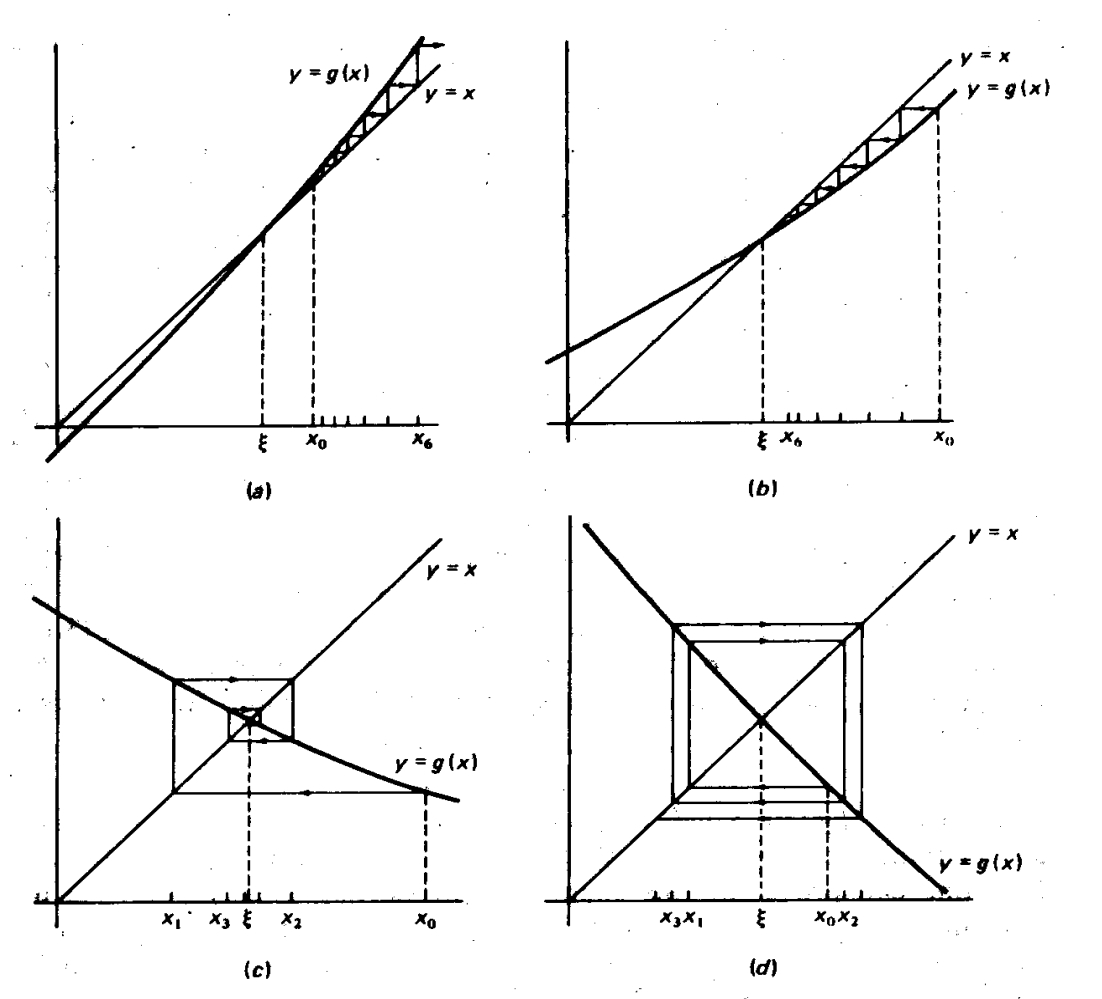
\includegraphics[width=0.6\textwidth]{figure/ne1_fixed_point_iteration_procedure.png}
    \caption{Fixed-point Iteration Procedure}
    \label{img:Fixed-point Iteration Procedure}
\end{figure}

\begin{theorem}{Convergence and Error of Fixed-Point iteration method}{convergence and Error of fixed-point iteration method}
    Assume that \\
    (1) $g,g'\in C[a,b]$;\\
    (2) $a \leqs g(x) \leqs b$;\\
    (3) $\lambda = \max_{a\leqs x\leqs b}|g'(x)|< 1$.\\
    Then \\
    (1) $x=g(x)$ has a unique solution $x^*$ in $[a,b]$.\\
    (2) For any choice of $x_0\in [a,b]$, with $x_{n+1}=g(x_n)$, $n=0,1,\dots$,
    \begin{align}
        \lim_{n\rightarrow \infty} x_n=x^*.
    \end{align}
    (3) We further have
    \begin{align}
        |x_n-x^*|\leqs \lambda^n |x_0-x^*|\leqs \frac{\lambda^n}{1-\lambda}|x_1-x_0|.
    \end{align}
\end{theorem}
\par
When using iterative methods, a natural question is when to stop the iteration?
Assume a positive number $\epsilon$ which is very small. Then, one of the following conditions may be used:\\
\textbf{Condition 1}: After each iteration check the inequality
\begin{align}
    |x_n-x_{n-k}|<\epsilon
\end{align}
for some fixed positive integer $k$. If this inequality is satisfied, 
the iteration can be stopped.\\
\textbf{Condition 2}: Another condition may be to check
\begin{align*}
    |f(x_n)|<\epsilon.
\end{align*}
This error is sometime called the residual error for the equation $f(x)=0$.


\section{Bisection Method}
Assume that $f(x)$ is continuous on a given interval $[a,b]$ 
and that is also satisfies $f(a)f(b)<0$
with $f(a)\neq 0$ and $f(b)\neq 0$.
Using the intermediate value theorem, we can see that the function $f(x)$
has at least one root in $[a,b]$.
We assume that there is only one root for the equation (\ref{eq:equations form})
in the interval $[a,b]$. The Bisection includes the following steps:\\
\textbf{Step 1}: Given an initial interval $[a_0,b_0]$, set $n=0$.\\
\textbf{Step 2}: Define $c_{n+1}=\frac{a_n+b_n}{2}$, the midpoint of the interval $[a_n,b_n]$.\\
\textbf{Step 3}:\\
If $f(a_n)f(c_{n+1})=0$, then $x^*=c_{n+1}$ is the root.\\
If $f(a_n)f(c_{n+1})<0$, then take $a_{n+1}=a_n$, $b_{n+1}=c_{n+1}$ and the root $x^*\in [a_{n+1},b_{n+1}]$.\\
If $f(a_n)f(c_{n+1})>0$, then take $a_{n+1}=c_{n+1}$, $b_{n+1}=b_n$ and the root $x^*\in [a_{n+1},b_{n+1}]$.
\\
\textbf{Step 4}: If the root is not obtained in step 3, then calculate the length of the new reduced interval $[a_{n+1},b_{n+1}]$.
If the length of the interval is less than a prescribed positive number $\epsilon$,
then take the midpoint of this interval ($x^*=\frac{a_{n+1}+b_{n+1}}{2}$) as the approximate root of the equation (\ref{eq:equations form}),
otherwise go to step 2. 
\par 
The following theorem gives the convergence and error for the bisection method.
\begin{theorem}{Convergence and Error of Bisection Method}{Convergence and Error of Bisection Method}
    Let $[a_0,b_0]=[a,b]$ be the initial interval, with $f(a)f(b)<0$.
    Define the approximate root as $x_n=\frac{b_{n-1}+a_{n-1}}{2}$.
    Then there exists a root $x^*\in [a,b]$ such that 
    \begin{align}
        |x_n-x^*|\leqs (\frac{1}{2})^n (b-a).
    \end{align} 
    Moreover, to achieve accuracy of $|x_n-x^*|\leqs \epsilon$, it suffices to take
    \begin{align}
        n\geqs \frac{\log(b-a)-\log\epsilon}{\log 2}.
    \end{align}
\end{theorem}


\section{Newton-Raphson Method}
The Newton-Raphson method, or Newton Method, is a powerful technique
for solving equations numerically. Like so much of the differential calculus,
it is based on the simple idea of linear approximation. The Newton Method,
properly used, usually homes in on a root with devastating efficiency.

\par
Let $x_0$ be a good estimate of $r$ and let $r = x_0 + h$. 
Since the true root is $r$, and $h = r - x_0$, 
the number $h$ measures how far the estimate $x_0$ 
is from the truth.
\par
Since h is 'small', we can use the linear (tangent line) approximation to
conclude that

\begin{align*}
    0=f(r)=f(x_0+h)\approx f(x_0)+hf'(x_0),
\end{align*}

and therefore, unless $f'(x_0)$ is close to $0$,
\begin{align*}
    h\approx -\frac{}{}
\end{align*}


\section{Secant Method}

\subsection{regula-falsi method}
The regula-falsi method is closely related to the bisection method. Recall the 
bisection method is to subdivide the interval $[a,b]$ in which the root lies into 
two parts, take the part of the interval which still holds the root and discard the other part of 
the interval. Although the bisection method always converges to the solution, the convergence is 
sometime very slow in the sense that if the root is very close to one of the boundary points(ie., $a$ and $b$)
of the interval. In such a situation, instead of taking the midpoint of the interval, 
we take the weighted average of $f(x)$ given by
\begin{align*}
    w=\frac{f(b)a-f(a)b}{f(b)-f(a)}.
\end{align*}
Similar to the iterative idea of Bisection Method, the regula-falsi method can defined as follows:\\
\textbf{Step 1}: Given an initial interval $[a_0,b_0]$, set $n=0$.\\
\textbf{Step 2}: Define $w_{n+1}=\frac{f(b_n)a_n-f(a_n)b_n}{f(b_n)-f(a_n)}$.\\
\textbf{Step 3}:\\
If $f(a_n)f(w_{n+1})=0$, then $x^*=w_{n+1}$ is the root.\\
If $f(a_n)f(w_{n+1})<0$, then take $a_{n+1}=a_n$, $b_{n+1}=w_{n+1}$ and the root $x^*\in [a_{n+1},b_{n+1}]$.\\
If $f(a_n)f(w_{n+1})>0$, then take $a_{n+1}=w_{n+1}$, $b_{n+1}=b_n$ and the root $x^*\in [a_{n+1},b_{n+1}]$.
\\
\textbf{Step 4}: If the root is not obtained in step 3, then calculate the length of the new reduced interval $[a_{n+1},b_{n+1}]$.
If the length of the interval is less than a prescribed positive number $\epsilon$,
then take the midpoint of this interval ($x^*=\frac{a_{n+1}+b_{n+1}}{2}$) as the approximate root of the equation (\ref{eq:equations form}),
otherwise go to step 2.


\section{Reference}
\begin{itemize}
    \item \href{https://www.math.iitb.ac.in/~baskar/book.pdf}{Introduction to Numerical Analysis ch4}
    \item \href{https://personal.math.ubc.ca/~anstee/math104/newtonmethod.pdf}{The Newton-Raphson Method}
    \item \href{}{J. H. Mathews and K. D. Fink: Numerical Methods using
    MATLAB ch2, Prentice Hall of India (PHI), 4th Edition, 2005} 
\end{itemize}




%%%%%%%%%%%%%%%Content%%%%%%%%%%%%%%%
% % \mainmatter % separat the number of toc and mainmatter
% \chapter*{Preface}

Notes mainly refer to following materials:


\begin{itemize}
    \item[*] Machine learning
    \begin{itemize}
        \item \href{https://www.cs.cornell.edu/courses/cs4780/2023sp/}{lecture notes from cornell}
        \item \href{https://www.cs.cmu.edu/~hn1/documents/machine-learning/notes.pdf}{lecture notes from cmu}
        \item \href{https://cs229.stanford.edu/main_notes.pdf}{lecture notes of CS229}
    \end{itemize}
    \item[*] Deep learning
    \begin{itemize}
        \item \href{https://udlbook.github.io/udlbook/}{understanding deep learning}
        \item \href{https://www.bilibili.com/video/BV1Wv411h7kN/?spm_id_from=333.337.search-card.all.click}{lecture video from Hongyi Lee}
        \item \href{https://cs231n.github.io/}{lecture notes from Stanford}
    \end{itemize}
    \item[*] Reinforcement learning
    \begin{itemize}
        \item \href{https://web.stanford.edu/class/cs234/modules.html}{lecture notes from stanford}
        \item \href{https://people.cs.umass.edu/~bsilva/courses/CMPSCI_687/Fall2022/Lecture_Notes_v1.0_687_F22.pdf}{lecture notes from umass}
    \end{itemize}
\end{itemize}







% \part{Mathematics}

% % !TEX root = ../notes_template.tex
\chapter{Discrete Math}\label{chp:discrete_math}


\section{Proof}

\begin{theorem}
\end{theorem}

\begin{solution}
By induction:
\end{solution}



\section{Quantifier}
\lipsum % dummy text - remove from real document

\section{Graph}
\citetitle{babaiGraphIsomorphismQuasipolynomial2016}
\cite{babaiGraphIsomorphismQuasipolynomial2016}

\section{Number theory}
Figure example
\begin{figure}[!ht]
    \centering
    \includegraphics[width=1\linewidth]{./figure/elliptic_curves.pdf}
    \caption{Elliptic curves \cite{childsUniversalComputationQuantum2009} }
\end{figure}


\section{Algorithm}
% \begin{center}
% \begin{minipage}{.9\linewidth}
% algorithm2e
% https://www.overleaf.com/learn/latex/Algorithms#The_algorithm2e_package
\begin{algorithm}[H]
    \SetKwInOut{Input}{input}
    \SetKwInOut{Output}{output}
    \Input{Integer $N$ and parameter $1^t$}
    \Output{A decision as to whether $N$ is prime or composite}
    \BlankLine
    \For{ $i = 1,2, \ldots, t$} {
        $a\leftarrow \qty{1,\dots,N_1}$\;
        \If{$a^{N-1} \neq 1 \mod{N}$}
    {\Return "composite"}
    }
    \Return "prime"
    \caption{Primality testing - first attempt}
    \label{alg:miller_rabin}
\end{algorithm}
% \end{minipage}
% \end{center}

% \part{Computer Science}
% % \input{./chapter/complexity.tex}
% % !TEX root = ../notes_template.tex
\chapter{Machine Learning}\label{chp:machine_learning}
\minitoc

\section{Regression}
% \gls{algorithm};
\subsection{Gradient descent}\label{sec:gradient_descent}
\gls{gd};
% \glsxtrshort{gd}

\section{Support Vector Machine}
\gls{svm};
% % \input{./chapter/algorithms.tex}

% \part{Physics}
% % !TEX root = ../notes_template.tex
\chapter{Quantum Mechanics}\label{chp:quantum_mechanics}
\minitoc

\section{Hamiltonian}
\gls{hamiltonian};
% \glsxtrshort{qm};

\section{Path Integral}
\gls{lagrangian}

\section{Quantum Field Theory}
\gls{qft};
% % \input{./chapter/quantum_field_theory.tex}

% % \begin{appendices}
% % % !TEX root = ../notes_template.tex
\chapter{Formulas}

\section{Gaussian distribution}\label{sec:gaussian_distribution}
\begin{Definition}[Gaussian distribution]\label{def:gaussian_distribution}
    \myindex{Gaussian distribution}
\end{Definition}

\begin{theorem}[Central limit theorem]\label{thm:central_limit_theorem}
\end{theorem}
% % \end{appendices}

% \backmatter

% %%%%%%%%%%%%%%% Reference %%%%%%%%%%%%%%%

% \printbibliography[heading=bibintoc]
% \printindex
\end{spacing}
\end{document}